\chapter{Implementación}
\label{chap:impl}

La figura \ref{fig:class-diagram} presenta el diagrama de clases del proyecto, que ha sido creada con la herramienta de generación automática de clases a partir de código de \textit{Visual Paradigm}\footnote{\url{https://www.visual-paradigm.com/}}.

Se ha diseñado la clase \texttt{Genetic\_Algorithm}, de la que heredan el resto de algoritmos, que contiene las variables y métodos comunes; esta clase define el tamaño y el número de las generaciones, parsea el fichero de datos, crea las generaciones\dots

De ella heredan tres clases; la implementación estándar del problema, \texttt{Standard}, la variante lamarckiana, \texttt{Lamarckian}, y la variante Baldwiniana, \texttt{Baldwinian}.

La clase \texttt{Individual}, que usan el resto de clases, representa a los individuos del algoritmo; estos individuos tienen un array que representa sus \textbf{cromosomas} (generados aleatoriamente) y otras herramientas, como funciones que permiten mutarlos conforme a una probabilidad, y un \textbf{fitness}, que indica cómo de óptimos son sus cromosomas.

Como \textbf{mecanismo de selección} se ha utilizado un \textbf{torneo binario}. En él, se eligen dos individuos al azar de la población actual y se devuelve aquél con menor fitness.

Como \textbf{mecanismo de reemplazo} se utiliza el \textbf{elitismo}; el mejor individuo de una generación pasa automáticamente a la siguiente, sustituyendo al peor de ésta.

Como \textbf{operador de mutación} se utiliza la \textbf{técnica del intercambio} adaptada para que dependa de una probabilidad. Cada individuo tiene una probabilidad de mutar como individuo y de que mute cada uno de sus cromosomas por separado.

\newpage

\vspace*{4em}

\begin{figure}[H]
  \centering
  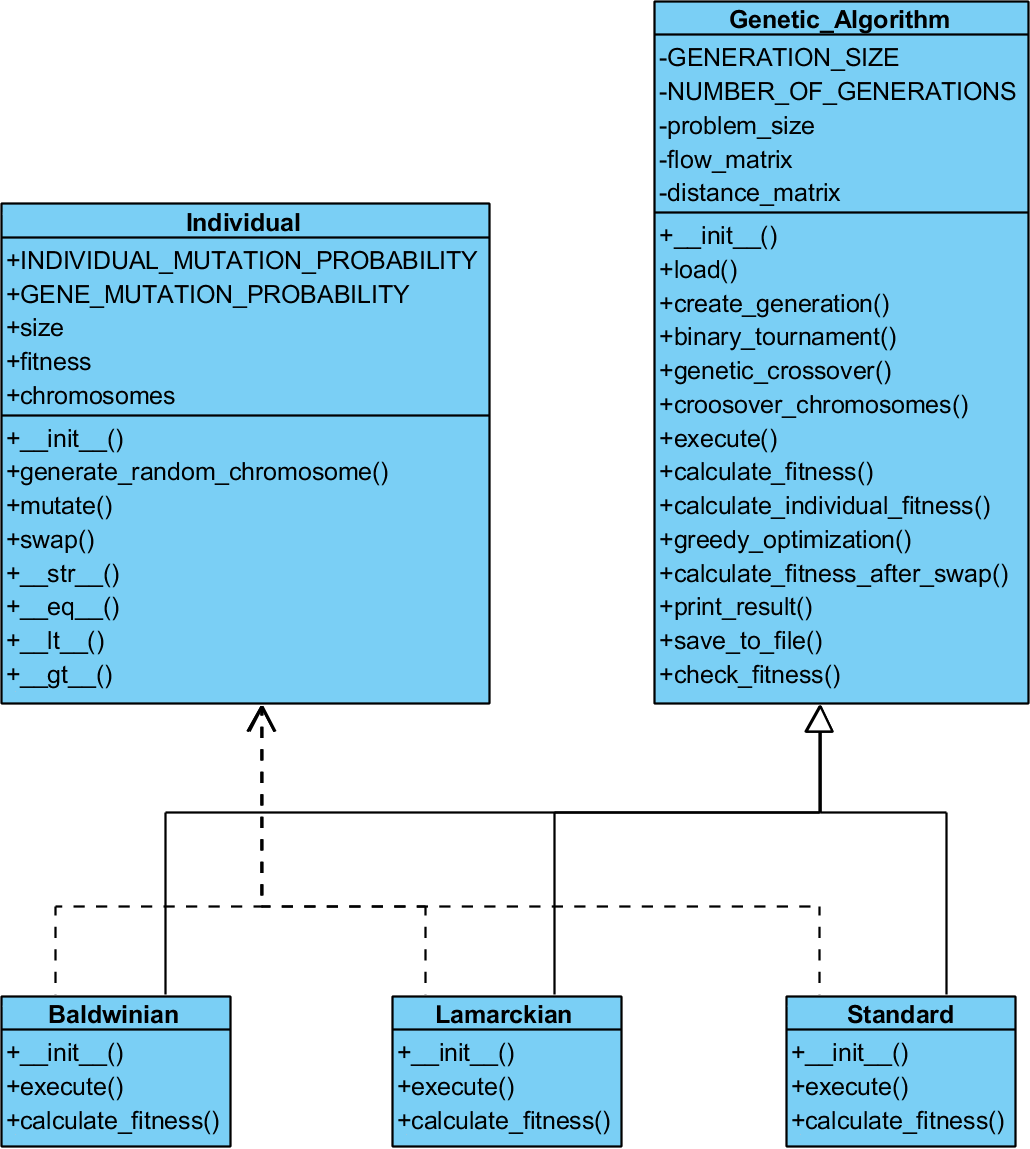
\includegraphics[width=1\textwidth]{../images/class-diagram}
  \caption{Diagrama de clases del proyecto}
  \label{fig:class-diagram}
\end{figure}

\newpage

Como \textbf{operador de cruce} se ha utilizado \textbf{recombinación en un punto}. Esta técnica permite cortar a ambos padres en un punto y recombinar sus trozos. La imagen \ref{fig:recombinacion-por-punto} representa este algoritmo, aunque específicamente en este problema hay que tener cuidado de no repetir sus cromosomas, pasando al siguiente número en caso de que ya exista.

\begin{figure}[H]
  \centering
  \captionsetup{justification=centering}
  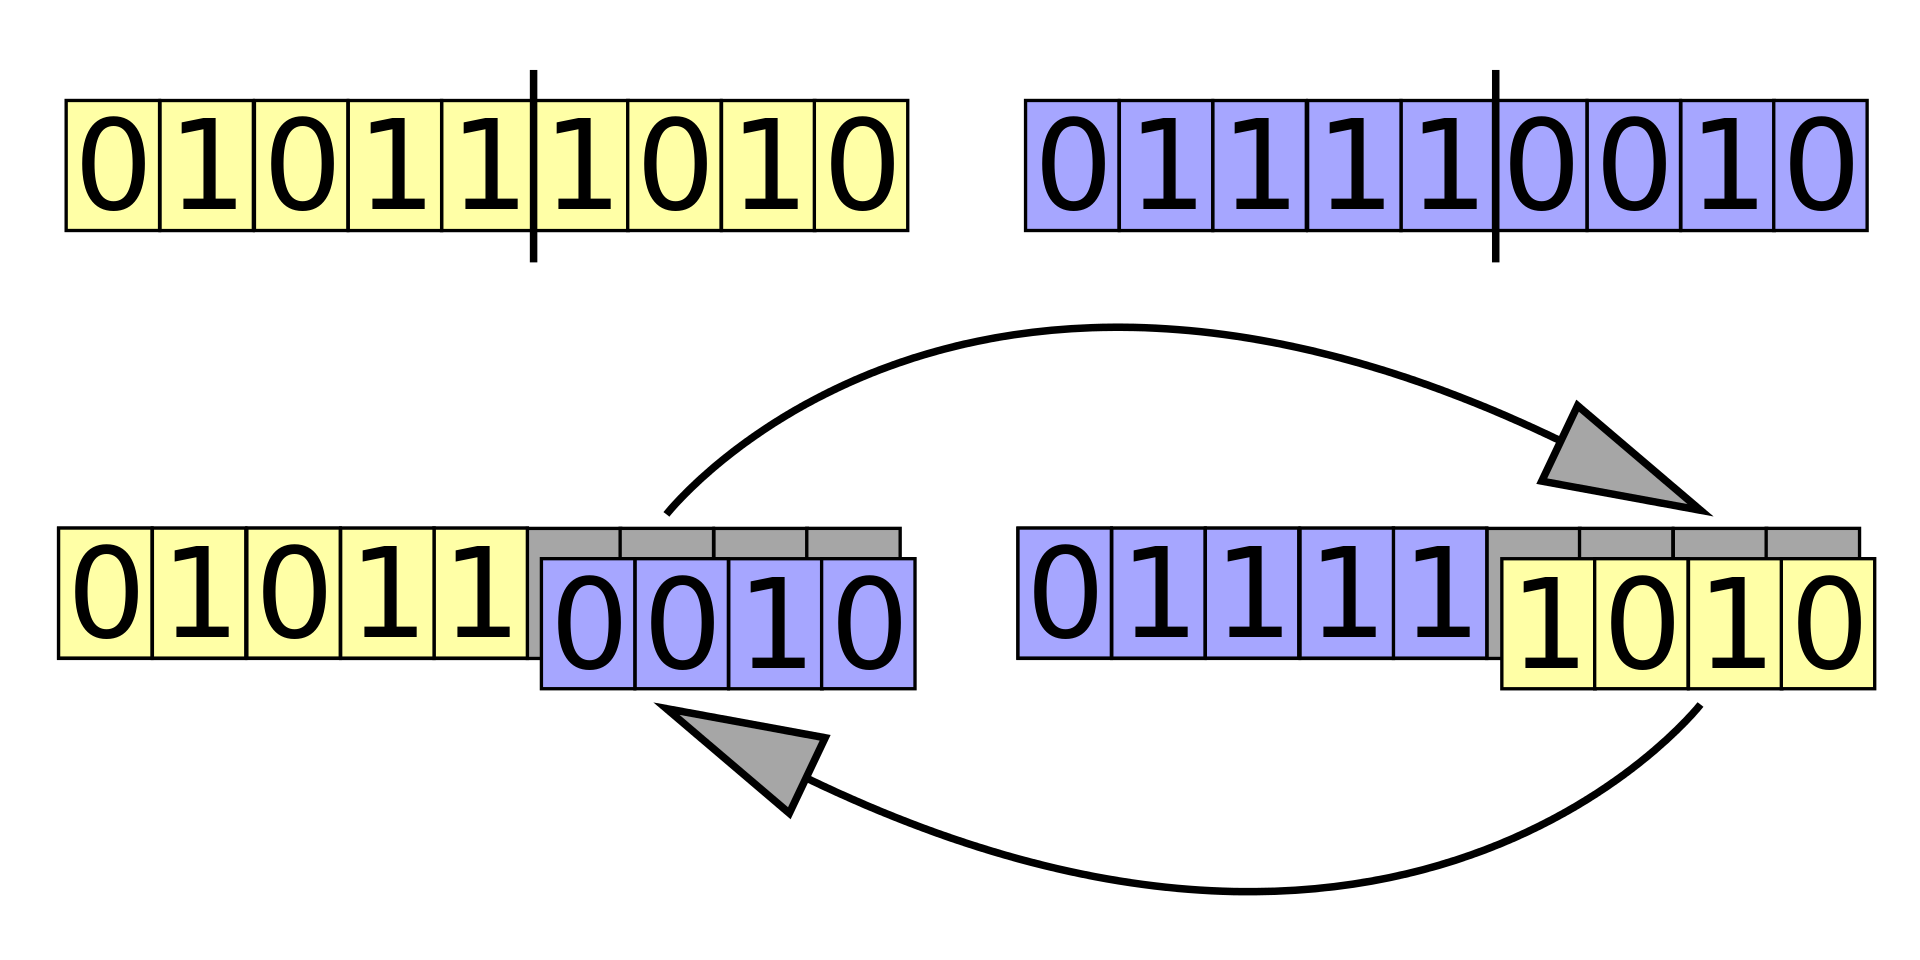
\includegraphics[width=0.5\textwidth]{../images/recombinacion-por-punto}
  \caption{Representación gráfica de la recombinación por punto}
  \small Referencia: Wikipedia.
  \label{fig:recombinacion-por-punto}
\end{figure}

Los tres algoritmos comparten la ejecución básica, ya que solo se diferencian en la manera de calcular el fitness de los individuos. En el listado \ref{lst:base-execution} puede verse el pseudocódigo de esta ejecución común.

\begin{lstlisting}[caption={Ejecución base de los algoritmos}, label={lst:base-execution}]
leer_fichero()
generacion_actual = crear_generacion()
generacion_actual.calcular_fitness()

for i=0..NUM_GENERACIONES:
    for j=0..TAM_GENERACION:
        padre1 = torneo_binario(generacion_actual)
        padre2 = torneo_binario(generacion_actual) && padre1 != padre2
        
        hijo1, hijo2 = recombinar(padre1, padre2)
        hijo1.mutar()
        hijo2.mutar()
        
        nueva_generacion.añadir(hijo1, hijo2)
        
    mejor = generacion_actual.obtener_mejor()
    nueva_generacion.sustituior_peor_por(mejor)
    generacion_actual = nueva_generacion
    generacion_actual.calcular_fitness()

    comprobar_que_el_mejor_no_se_repite_o_reinicializar(mejor)

return generacion_actual.obtener_mejor()
\end{lstlisting}

En la linea 21, la única no explicada anteriormente, se comprueba que el mejor individuo de la población no lleva repitiéndose más veces que las permitidas, y de ser así reinicia la población conservando el mejor individuo de la anterior.

\section{Algoritmo estándar}

De las tres implementaciones de la que consta la práctica, el algoritmo estándar fue el primero que se programó. Su fitness es el más sencillo, ya que basta con aplicar la fórmula \ref{formula:sum} explicada en la introducción.

\section{Variantes evolutivas}

La técnica de optimización local aplicada es un algoritmo \textit{greedy 2-opt}. El fragmento de pseudocódigo \ref{lst:greedy-2opt} muestra cómo funciona.

\begin{lstlisting}[caption={Optimización greedy 2-opt}, label={lst:greedy-2opt}]
S = candidato inicial con coste c(S) 
mejor = S
for i=1..n:
    for j=i+1..n:
        T = S tras intercambiar i con j 
        if c(T) < c(S):
            S=T
return S
\end{lstlisting}

Se ha simplificado con respecto a la versión propuesta en el guión de prácticas eliminando el bucle \texttt{while}, ya que es prácticamente imposible que tras iterar cuadráticamente sobre el tamaño del problema \texttt{S} y \texttt{T} terminen siendo iguales, y tras realizar pruebas se comprobó que esto nunca sucede, por lo que se decidió eliminar de la implementación.

Por otro lado Python, por ser un lenguaje interpretado, funciona especialmente lento en comparación a otros lenguajes compilados, por lo que se ha dedicado un esfuerzo extra en intentar optimizar todo lo posible el algoritmo. Concretamente, y como fue propuesto en clase por el profesor Berzal, se ha diseñado una función específica para recalcular el fitness de los individuos tras intercambiar sus cromosomas (línea 5 del listado \ref{lst:greedy-2opt}), modificando solo los valores que han cambiado. Así, se ha conseguido reducir la complejidad de esa función en concreto de $O(n^2)$ a $O(n)$. 

\subsection{Variante lamarckiana}

Esta variante está basada en la teoría evolutiva del naturalista francés \textbf{Jean-Baptiste Lamarck} (1744-1829), quien afirmaba que las mejoras fisiológicas que obtenía un individuo a lo largo de su vida  quedaban grabadas en sus genes, por lo que sus descendientes adquirían esta mejoras en su código genético.

Así, tras obtener un individuo optimizado con la función presentada en el litado \ref{lst:greedy-2opt}, el individuo original el sustituido por su versión mejorada.

\subsection{Variante baldwiniana}

Esta variante está basada en la teoría evolutiva del psicólogo estadounidense \textbf{James Mark Baldwin} (1861-1934), quien afirmaba que las mejoras fisiológicas de un individuo obtenidas a lo largo de su vida no se graban en sus genes, por lo que su descendencia no las obtiene.

Así, tras aplicar una optimización local en cada generación, éstas no se usan para generar la siguiente población, sino que \textit{mueren} con sus individuos.